\documentclass{article}
\usepackage[utf8]{inputenc}
\usepackage{url}
\usepackage{graphicx}
\graphicspath{ {./images/} }
\usepackage{pdfpages}
\usepackage{booktabs}
\usepackage{xcolor,colortbl}
\usepackage{geometry}
\geometry{
 a4paper,
 total={170mm,257mm},
 left=20mm,
 top=20mm,
}

\usepackage{caption}
\usepackage{subcaption}

\usepackage{fullpage}
\usepackage{times}
\usepackage{fancyhdr,graphicx,amsmath,amssymb}
\usepackage[ruled,vlined]{algorithm2e}

%%%%%%%%%%%%%%%%%%%%%%%%%%%%%%%%%%%%%%%%%%%%%%%%%%

\title{Semester Plan \& Progress Reports}
\author{Luke Kurlandski}
\date{08/2022 - 12/2022}

\begin{document}

\maketitle

\section*{Check-in 0 (08/29/2022)}

Goal for the semester is to develop a research objective to work on for the RPA in Spring 2023.

\subsection*{Plan (09/08/2022)}

\begin{itemize}
	\item By the end of September (09/30/22)
	\begin{itemize}
		\item Find a research topic to focus on. Ideas include
		\begin{itemize}
			\item Practical black-box evasion attacks within the problem space (directly modifying the malware itself and ensuring its functionality remains unchanged)
			\item Poisoning attacks on malware classifiers
			\item Code modeling/NLP techniques applied on malware source code, opcode, etc.
			\item In general, focus on PE malware (90\% of malware) and static malware research (more suited to my current skillset)
		\end{itemize}
		\item Obtain a computer from Charles.
		\item Read other student's RPAs.
	\end{itemize}
	\item By the end of October (10/31/22)
	\begin{itemize}
		\item Determine research objective within topic.
		\begin{itemize}
			\item What results I want to show
			\item What conclusions I want to make
		\end{itemize}
		\item Literature review month.
	\end{itemize}
	\item By the end of November (11/30/22)
	\begin{itemize}
		\item Develop a methodology to achieve objective.
		\begin{itemize}
			\item Experiments to run
			\item Determine other knowledge needed
		\end{itemize}
		\item Literature review month.
	\end{itemize}
	\item By the end of December (12/31/22)
	\begin{itemize}
		\item Possibly have some preliminary results
		\item Adjust methodology as needed
		\item Rinse and repeat
	\end{itemize}
	\item Semester-long goals/activities
	\begin{itemize}
		\item Read as much as possible.
		\item Take notes.
		\item Pass classes.
		\item Attend dissertation defenses, research talks, etc.
		\item Produce one-page progress reports each month.
	\end{itemize}
\end{itemize}

\section*{Check-in 1 (10/12/2022)}

\subsection*{Progress Report}

For the most part, I am slightly ahead of schedule in terms of developing an idea to work on. However, it is a hard idea and remains to be seen whether or not it will work. The poster for AI@RIT serves as the more conceptually-rigorous component of this month's updates. I did not read other student's RPAs because it seemed like that might be more beneficial to save for either December or January.

\subsection*{Plan (10/12/2022)}

\begin{itemize}
	\item By Monday 10/31/22
	\begin{itemize}
		\item Proof-of-concept example demonstrating that rewriting snippets can make them less suspicious-looking.
		\item Initial benign-looking and malicious-looking nonparallel corpora.
		\item Emphasize literature review.
	\end{itemize}
	\item By Monday 11/21/22
	\begin{itemize}
		\item Initial unsupervised translation system (denoising and backtranslation).
		\item Refined nonparallel corpora (function segmentation, different explanation algorithms).
		\item Assess whether switching to Android malware would be productive.
		\item Emphasize literature review.
		\item Check-in II.
	\end{itemize}
	\item By Monday 12/19/22
	\begin{itemize}
		\item Refined translation system (pretrained LLM encoder/decoder).
		\item Setup adversarial attack simulation.
		\item Attain preliminary results.
	\end{itemize}
\end{itemize}

\pagebreak

\section*{Check-in 2 (11/21/2022)}

\subsection*{Progress Report}

For the past several weeks, we have been investigating whether or not an adversarial attack that rewrites malware's source code could be successful. To determine whether such an attack could actually fool a classifier, we modify the bytes of PE malware inside of the PE file's .text section and run the perturbed malware through a raw-byte classifier to see if it evades detection. Preliminary results indicate that using random bytes or baseline/padding bytes does not produce perturbed malware that can evade a classifier. However, using bytes from the .text section of a benign executable has been successful to some degree. At the very least, this confirms that the source code within malware is meaningful to the classifier. If we can figure out a way to make malicious source code appear benign, we should be able to make at least some malware evade classification.

We want to have an understanding of how many bytes in the malware we would need to change to launch a successful attack. Therefore, it makes sense to repeatedly select a small chunk of bytes from a malware sample, perturb it, and evaluate the perturbed sample against the classifier. There are two main aspects to consider when performing these incremental substitution experiments. The first is how to select bytes from the malicious example to be replaced at every iteration. We experiment with selecting chunks of the malicious executable in order, randomly, and according to how suspicious an explanation algorithm considers the chunk. The second aspect to consider is how to select bytes from the benign sample to use as a replacement. We experiment with selecting the chunks of the benign executable that correspond to the offset of the chunk selected from the malicious executable and selecting chunks which are the least suspicious according to an explanation algorithm.

Preliminary results on a poorly-learned model seemed to suggest that the SHAP explanation algorithm was successful at identifying suspicious chunks of malware and replacing these suspicious chunks was an efficient way to produce perturbed malware that evades a classifier.

To build upon this, we use a pretrained low-memory ``Global Channel Gating'' MalConv model trained extensively on a large corpus of malicious and benign executables. Running experiments on this model produces some interesting results, which partially contradict our previous findings (Figure 1). First, the overall evasion rate of the perturbed malware was slightly lower than in our initial experiments. Second, the relationship between the percentage of perturbed malware examples classified as benign and the amount of bytes modified was more linear, rather than logarithmic. Third, selecting the most suspicious chunk of malware for replacement, instead of a random chunk or each chunk in order, only slightly improved the evasion rate. Fourth, selecting the least benign chunk from the malicious executable slightly improves the evasion rate compared to selecting the corresponding chunk.

The second, third, and fourth observations are somewhat concerning. Ideally, we hoped there would be a more logarithmic relationship between the evasion rate and the proportion of bytes being replaced because this would mean that less bytes would need to be modified as part of the attack. We also anticipated more significant differences between the different methods of selecting bytes from the malicious sample to be replaced and more significant differences between the methods for selecting bytes from the benign sample to replace with. These observations may indicate that the explanation algorithm is not very successful at identifying which regions are suspicious-looking and which are not. 

My idea of using machine translation to rewrite malware rests on the premise that we can identify which snippets of code are benign-looking and which are malicious-looking. With that in mind, I believe I need to spend more time on this aspect of the research and verify that the explanation algorithms provide useful information.

\pagebreak

\subsection*{Plan (11/21/2022)}

The plan I created last check-in was definitely overly ambitious. Here is a loose plan moving forward.

\begin{itemize}
	\item By Monday 12/05/22
	\begin{itemize}
		\item Find some evidence that the results from an explanation algorithm are useful
		\item Build nonparallel corpora using explanation methods
	\end{itemize}
	\item By Monday 12/19/22
	\begin{itemize}
		\item Build a pseudo NMT model that produces syntactically correct x86
		\item Check-in 3
	\end{itemize}
	\item By Monday 01/16/22
	\begin{itemize}
		\item Other research goals TBD
		\item RPA Related Work first draft	
		\item RPA committee members list
	\end{itemize}
\end{itemize}

\pagebreak

\begin{figure}[ht]
	\centering
	\begin{subfigure}{.5\textwidth}
		\centering
		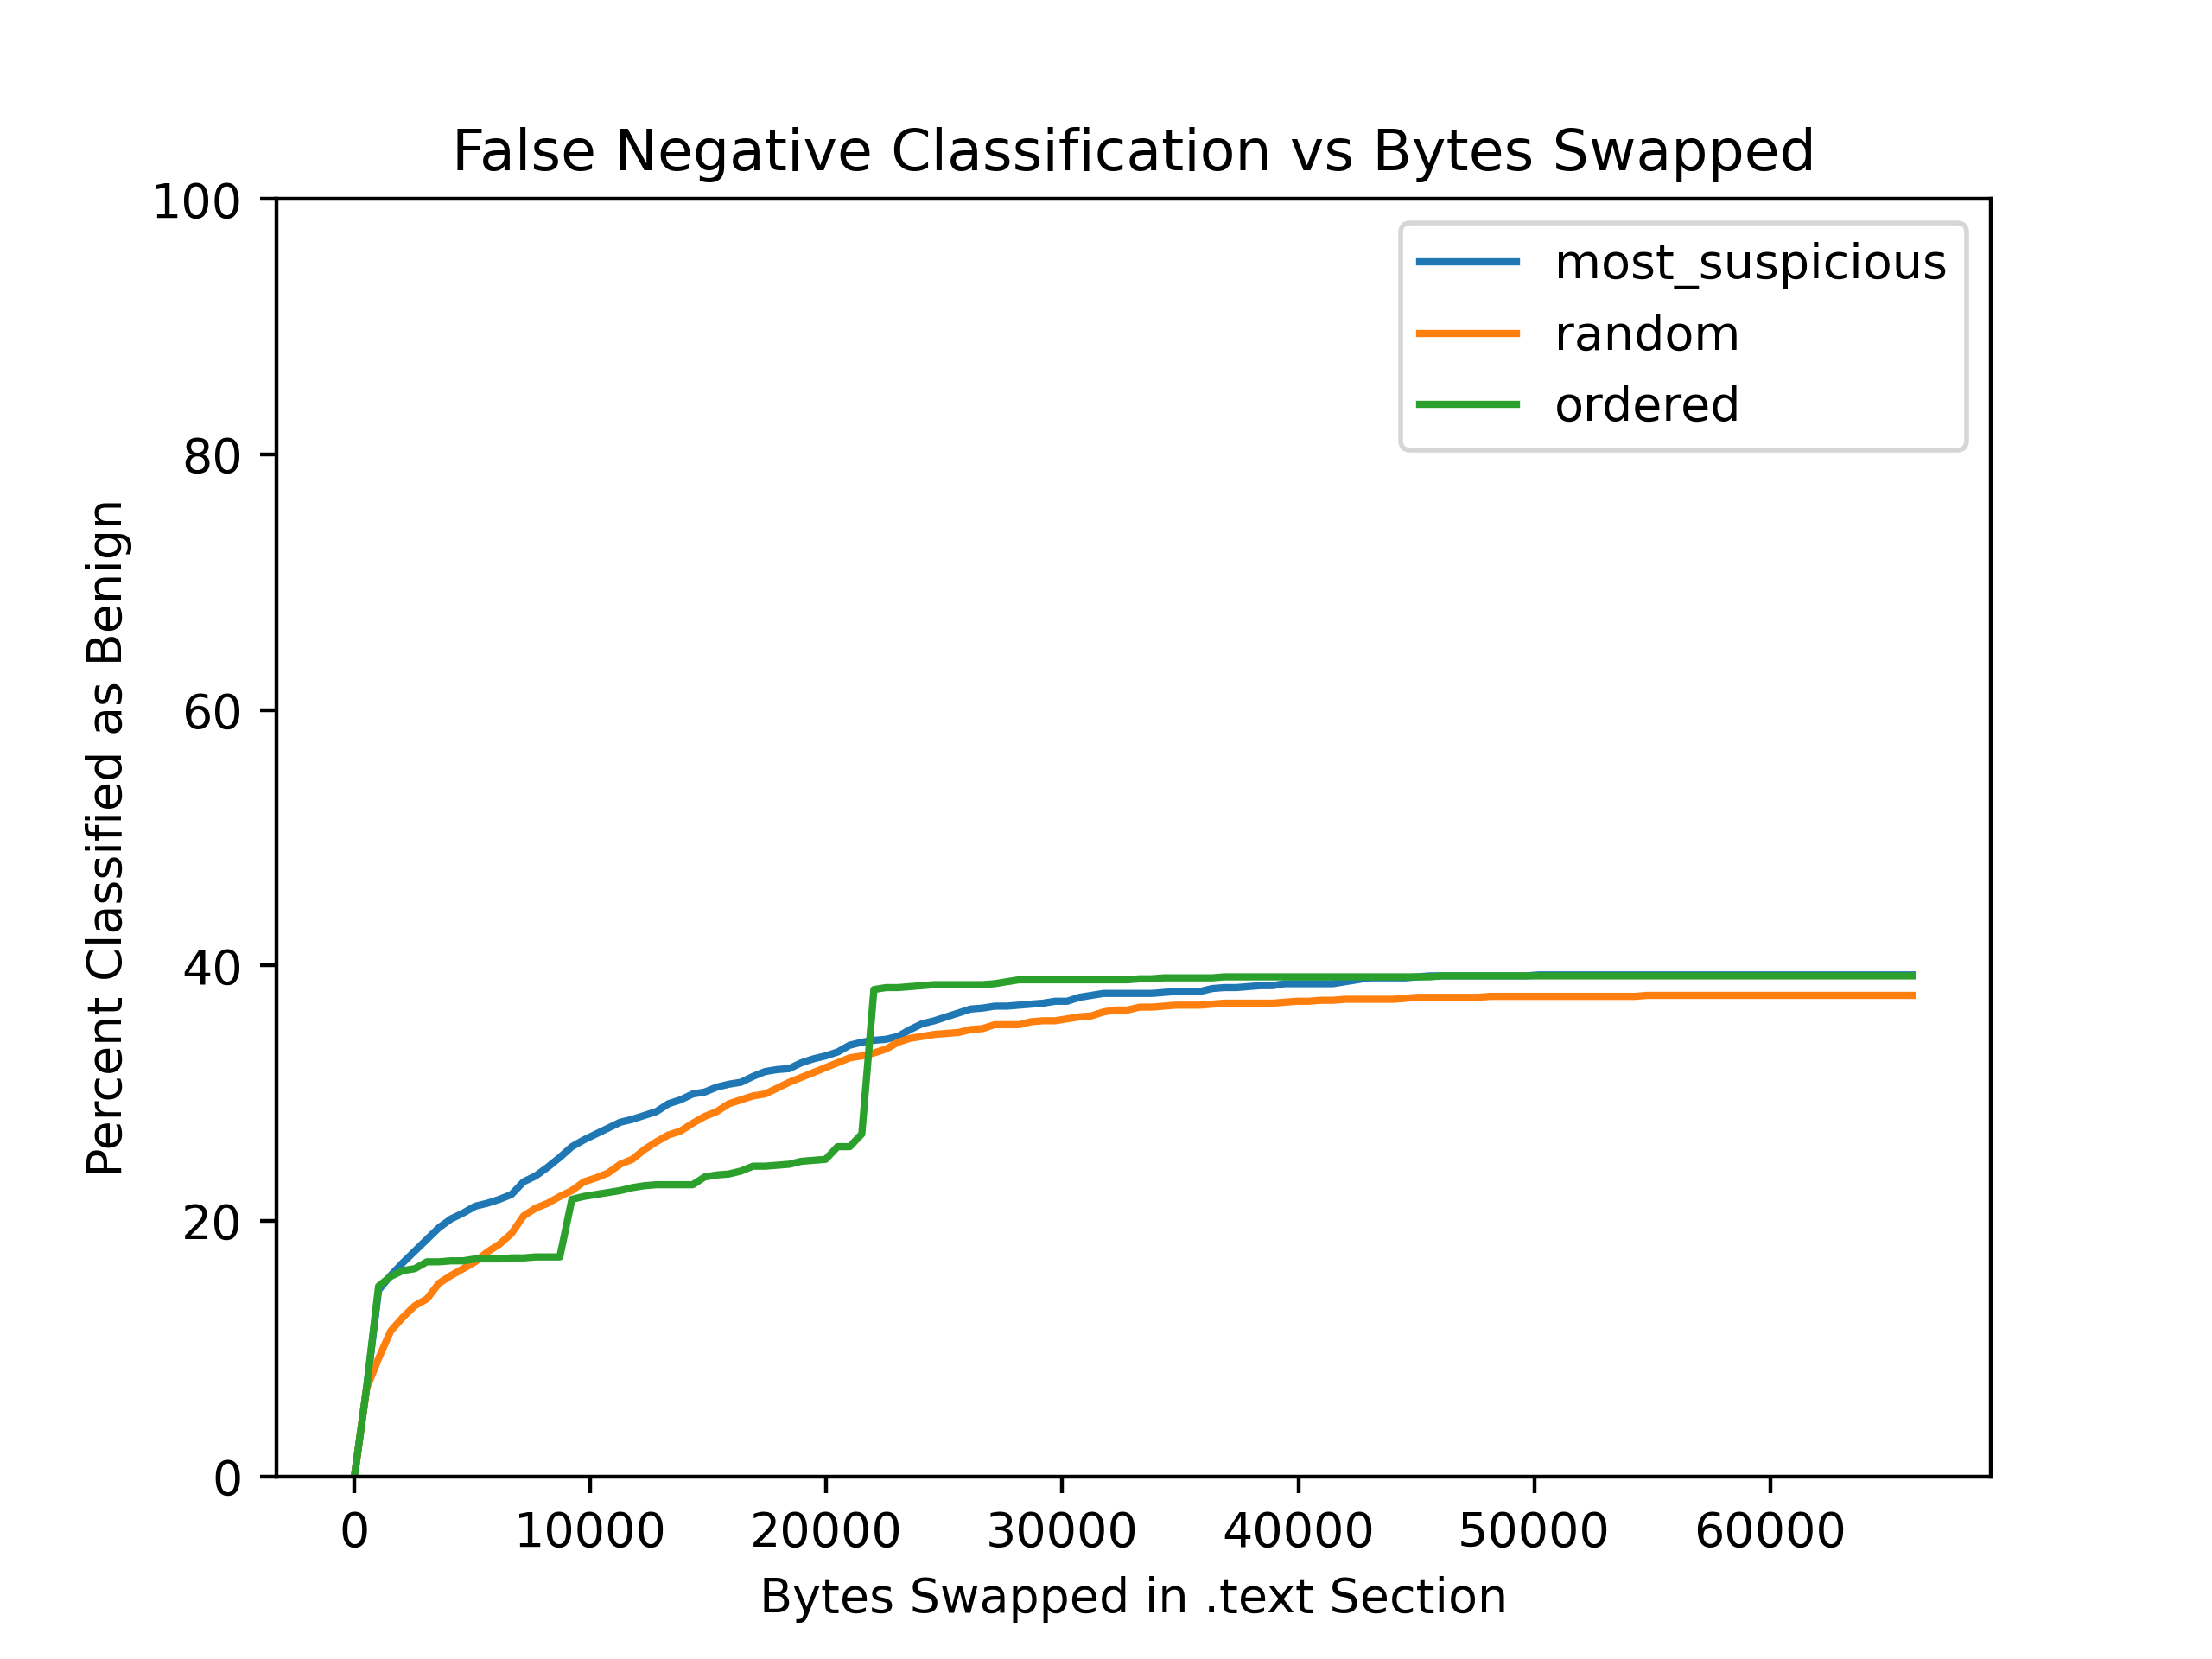
\includegraphics[scale=.5]{./figures/plan/2/corresponding-absolute.png}
		\caption{Corresponding-benign swap method (absolute).}
	\end{subfigure}%
	\begin{subfigure}{.5\textwidth}
		\centering
		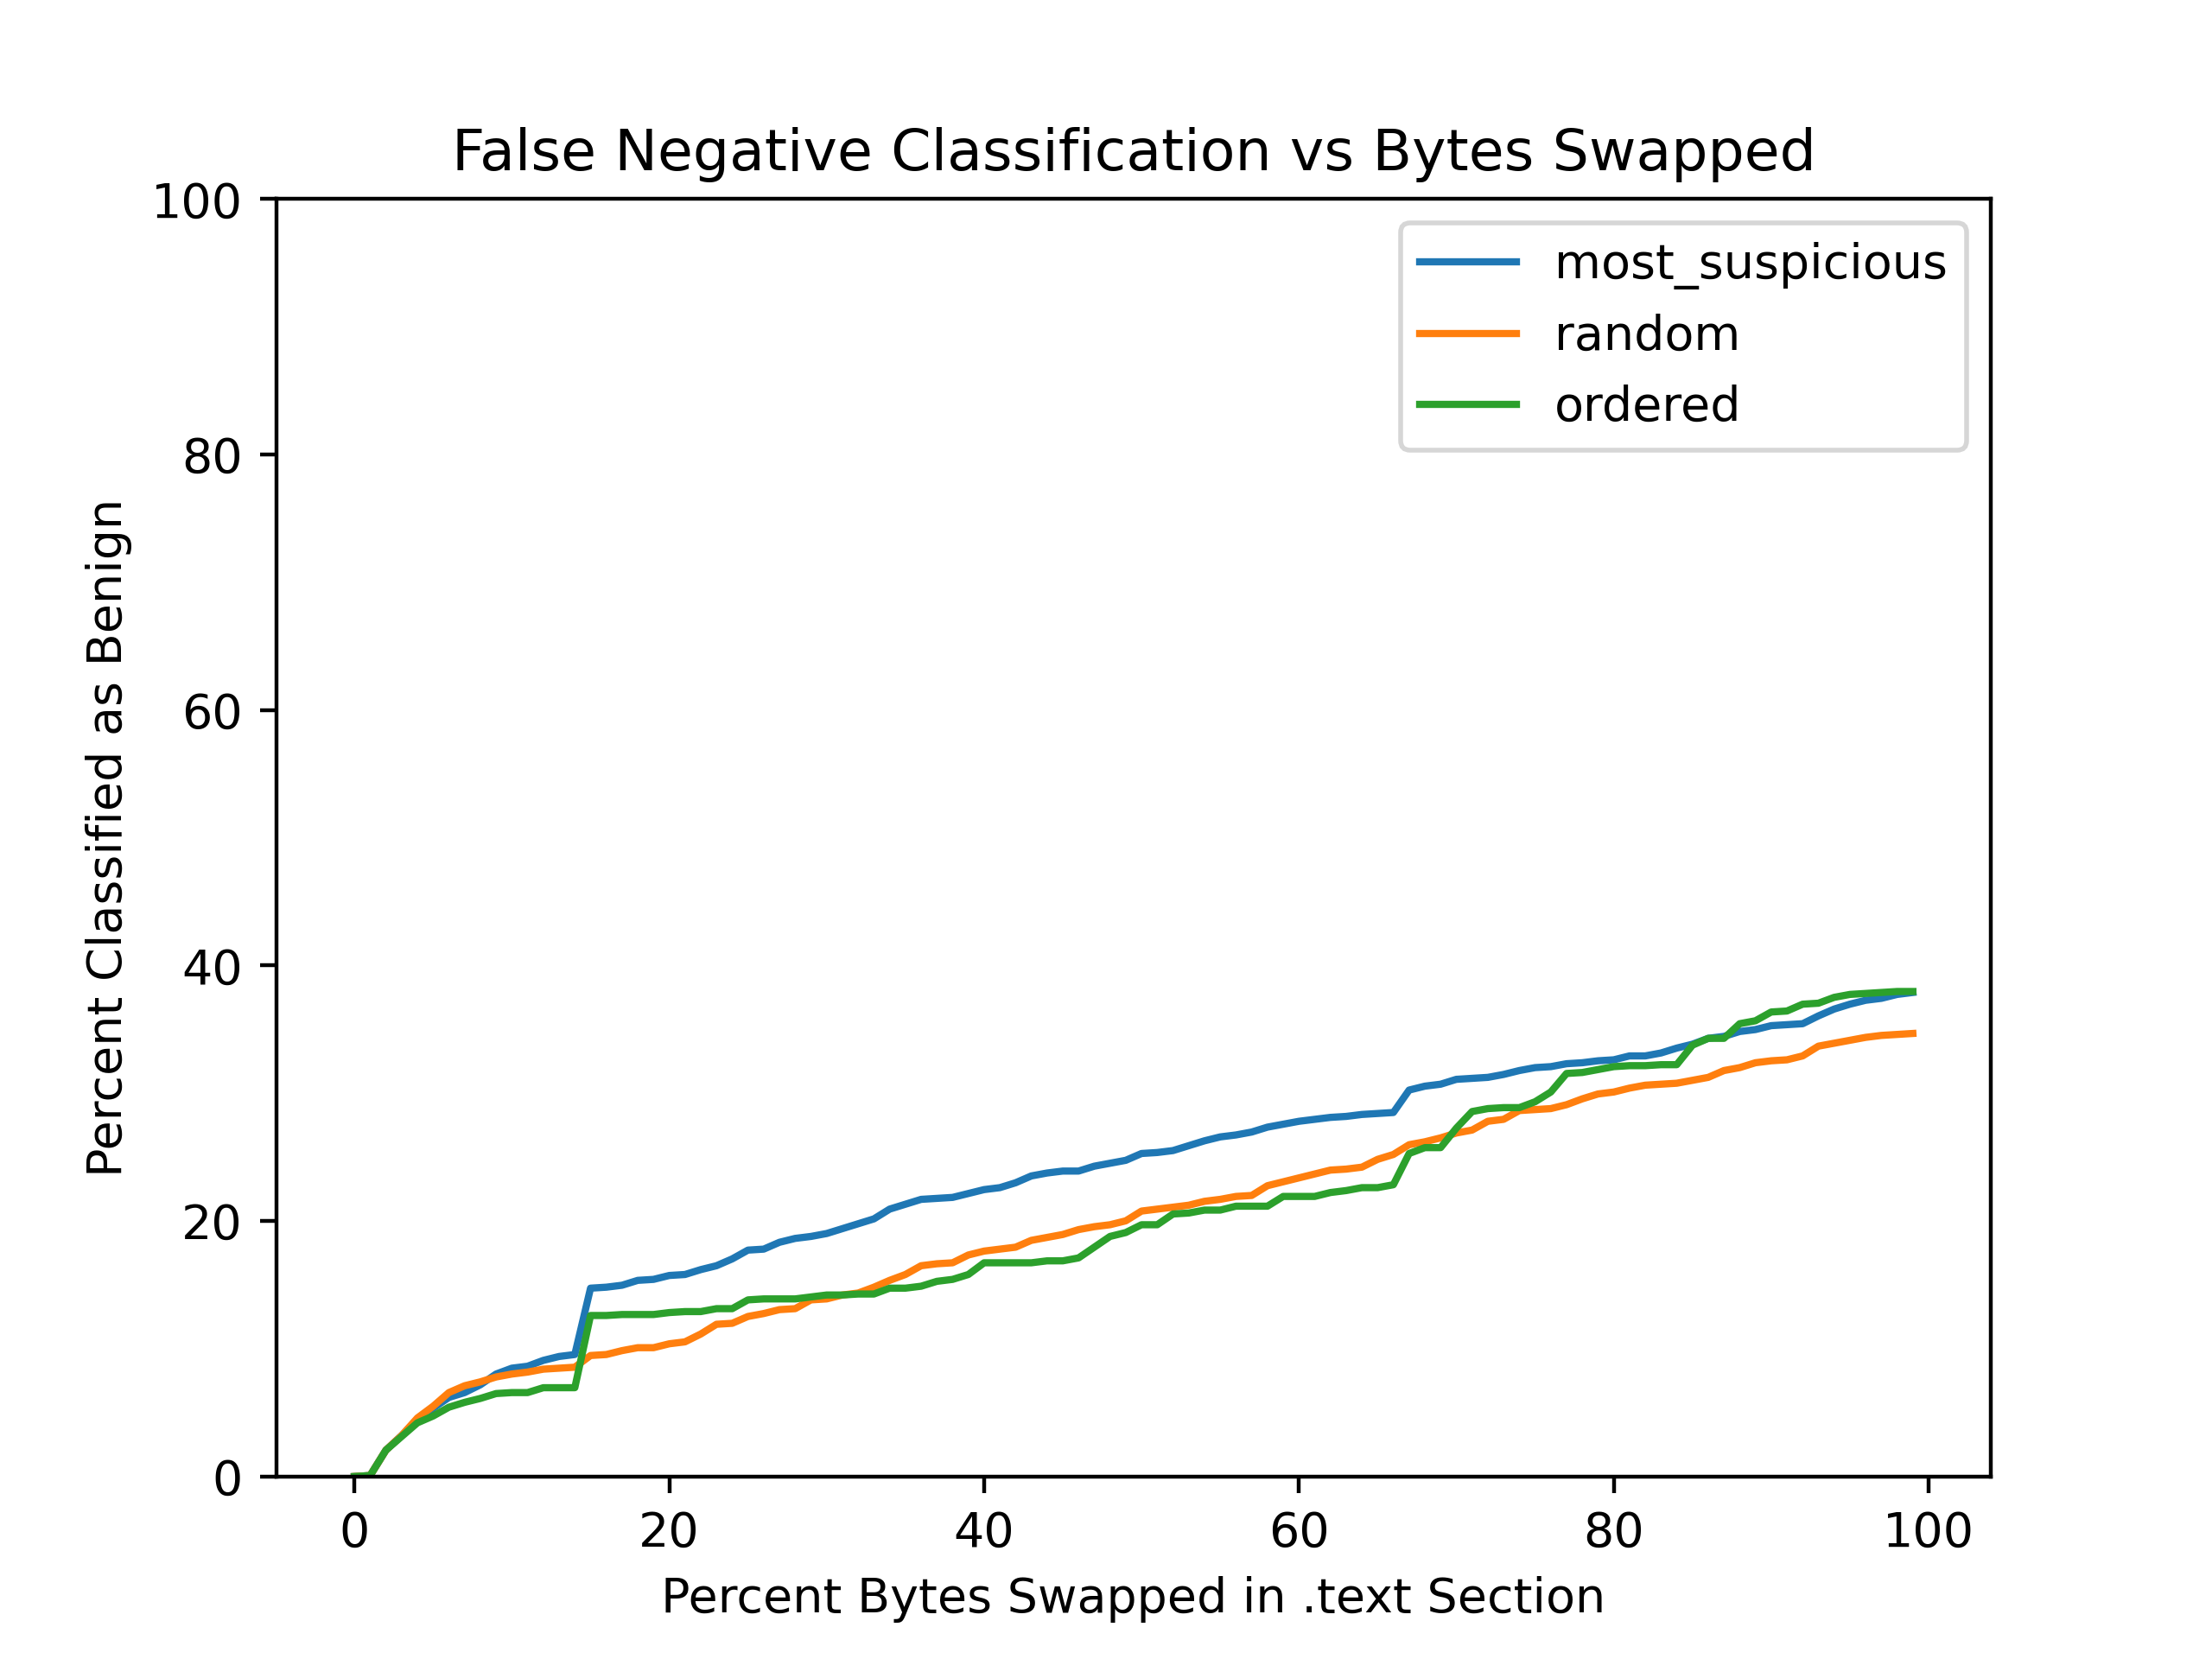
\includegraphics[scale=.5]{./figures/plan/2/corresponding-proportion.png}
		\caption{Corresponding-benign swap method (proportion).}
	\end{subfigure}\\
	\begin{subfigure}{.5\textwidth}
		\centering
		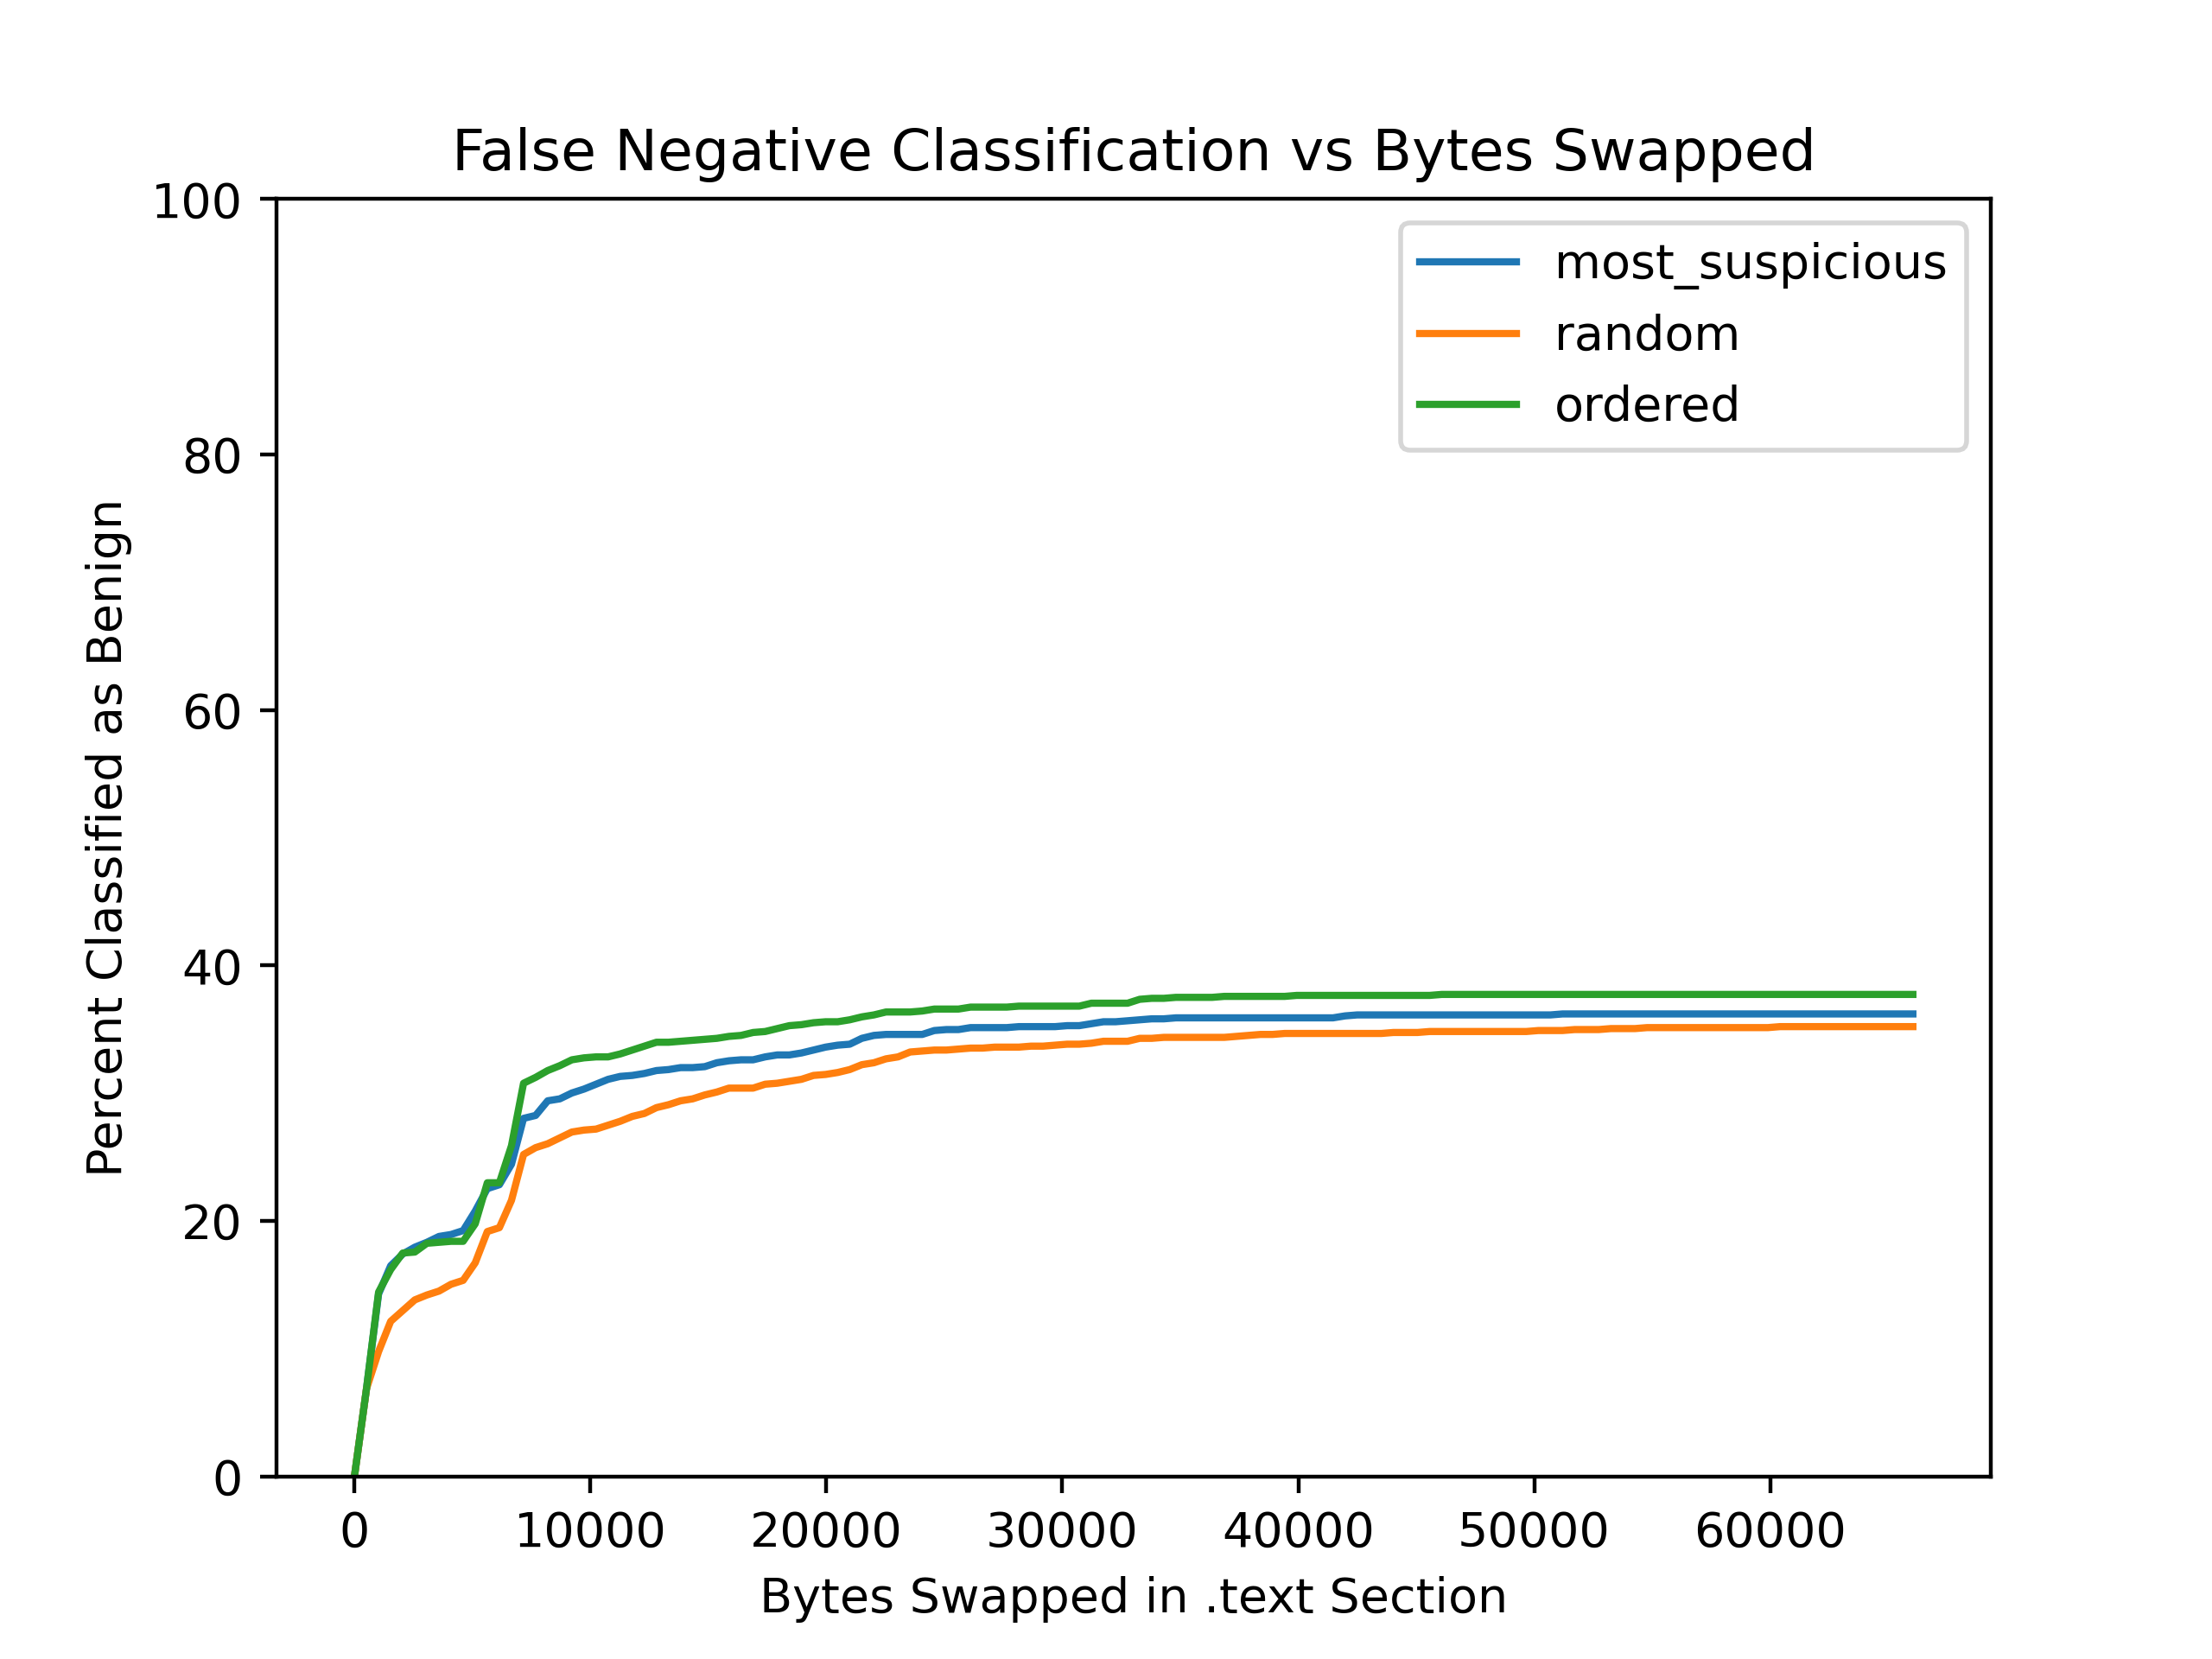
\includegraphics[scale=.5]{./figures/plan/2/least-absolute.png}
		\caption{Least-suspicious-benign swap method (absolute).}
	\end{subfigure}%
	\begin{subfigure}{.5\textwidth}
		\centering
		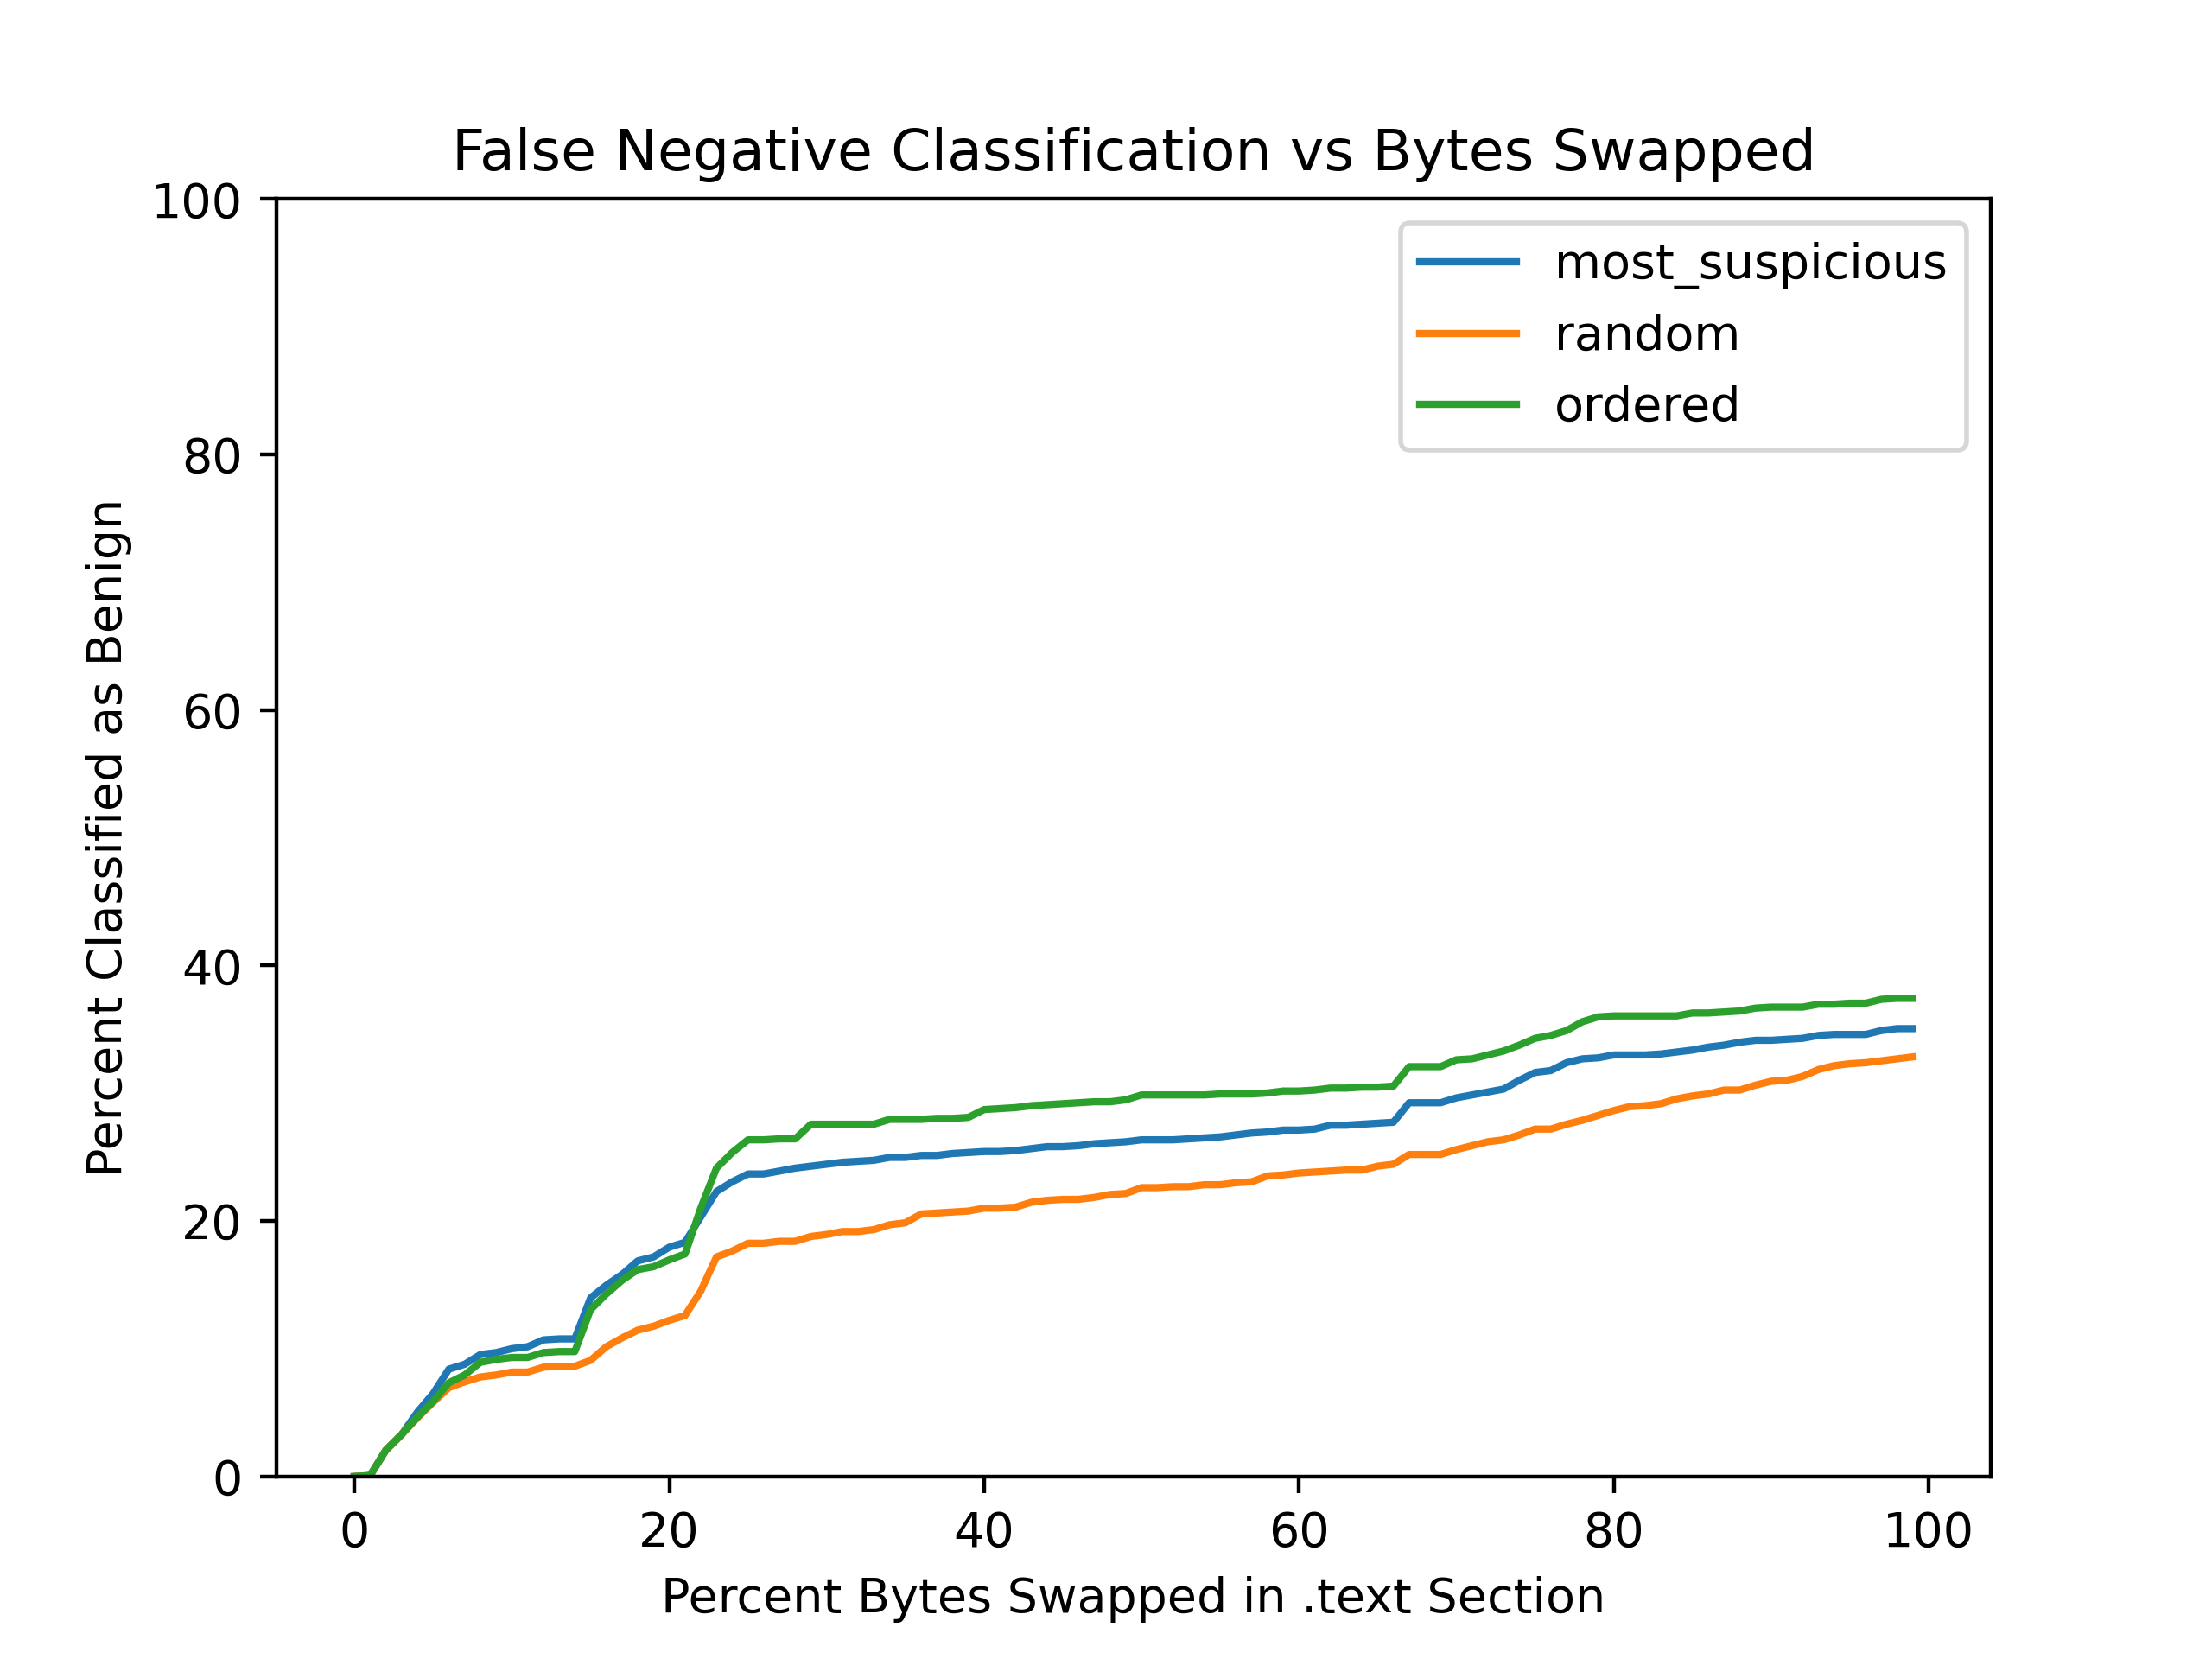
\includegraphics[scale=.5]{./figures/plan/2/least-proportion.png}
		\caption{Least-suspicious-benign swap method (proportion).}
	\end{subfigure}
	\caption[Theoretically, the three lines in each individual plot should achieve the same evasion rate. The fact that they do not is because of a bizarre feature/bug in the original implementation of the Global-Channel-Gating MalConv. It is not a major issue, but I have been in contact with Edward Raff about the feature/bug on GitHub (https://github.com/NeuromorphicComputationResearchProgram/MalConv2/issues/6)]{False negative rate vs the amount of bytes swapped using different methods of incrementally perturbing a malicious executable. There are four subfigures. Subfigures (a) and (b) use the chunk of bytes from the benign executable that corresponds to the offset of the chunk of bytes from the malicious executable that was selected for replacement. Subfigures (c) and (d) use the next least suspicious chunk of bytes selected from the benign executable at every swap iteration. Each subfigure displays three lines. Each line indicates the false negative rate for a different method of selecting chunks to substitute from the malicious file. The three different methods are: `most\_suspicious', which selects the most suspicious chunk from the malware for modification, `random', which selects a random chunk, and `ordered', which selects chunks in the order they appear in the original malicious executable.\footnotemark}
\end{figure}

\footnotetext{Theoretically, the three lines in each individual plot should achieve the same evasion rate. The fact that they do not is because of a bizarre feature/bug in the original implementation of the Global-Channel-Gating MalConv. It is not a major issue, but I have been in contact with Edward Raff about the feature/bug on GitHub (https://github.com/NeuromorphicComputationResearchProgram/MalConv2/issues/6)}

\end{document}